\documentclass[tikz,border=10pt]{standalone}
\begin{document}
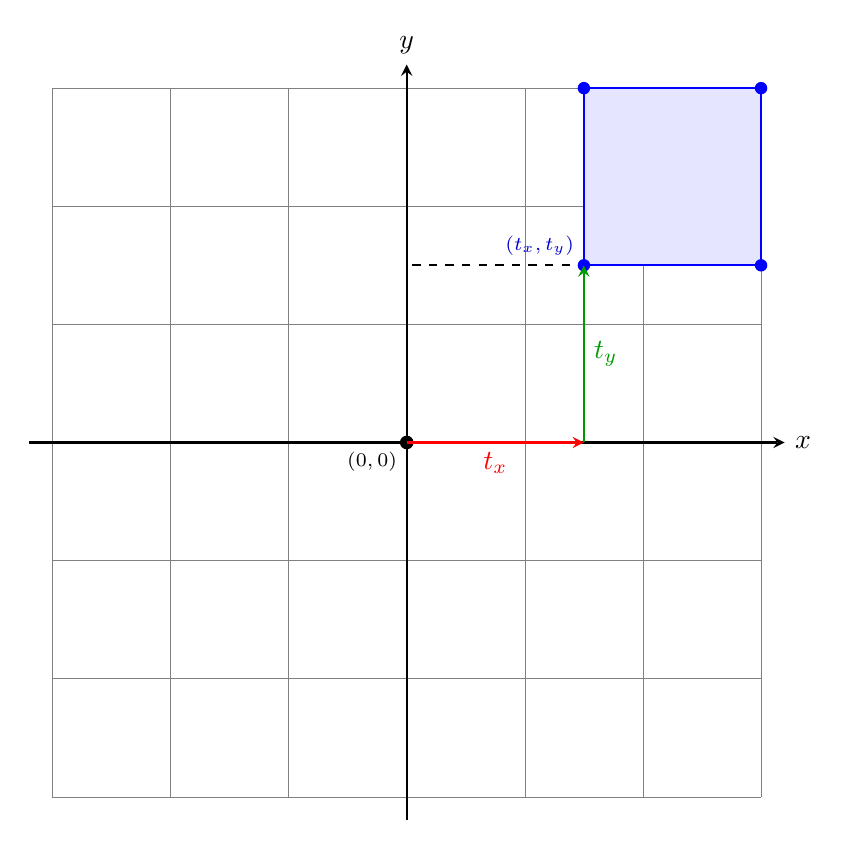
\begin{tikzpicture}[>=stealth, scale=1.5]

    % 6x6 Grid (from -3 to 3 on both axes)
    \draw[help lines, step=1] (-3,-3) grid (3,3);

    % Axes
    \draw[->, thick] (-3.2,0) -- (3.2,0) node[right] {$x$};
    \draw[->, thick] (0,-3.2) -- (0,3.2) node[above] {$y$};

    % Parameters for square size and translation
    \def\side{1.5}
    \def\tx{1.5}
    \def\ty{1.5}

    % Original Dashed Square (Bottom-left at 0,0)
    \draw[dashed, thick] (0,0) rectangle (\side,\side);
    \filldraw[black] (0,0) circle (1.5pt) node[below left, font=\scriptsize] {$(0,0)$};

    % Translated Solid Blue Square (Bottom-left at tx, ty)
    \filldraw[fill=blue!10, draw=blue, thick] (\tx,\ty) rectangle ({\tx+\side},{\ty+\side});
    
    % Corner dots for the blue square
    \foreach \x/\y in {\tx/\ty, {\tx+\side}/\ty, {\tx+\side}/{\ty+\side}, \tx/{\ty+\side}} {
        \fill[blue] (\x,\y) circle (1.5pt);
    }
    
    % Label new bottom-left coordinate
    \node[above left, font=\scriptsize, text=blue!80!black] at (\tx,\ty) {$(t_x, t_y)$};

    % Translation Vectors tracing the path from the bottom-left corner
    \draw[->, red, thick] (0,0) -- (\tx,0) node[midway, below] {$t_x$};
    \draw[->, green!60!black, thick] (\tx,0) -- (\tx,\ty) node[midway, right] {$t_y$};

\end{tikzpicture}
\end{document}